\chapter{Evaluation}

\pengcheng{for each experiment, 4 paragraphs: 1. why are we doing the experiment and what is to show; 2. description of the experimental procedure; 3. describe the results; 4. draw a conclusion}

We present the preliminary evaluation results of the FPsPIN implementation.  We have two results presented here: \emph{theoretical} analysis of latencies of various fast-path components and \emph{end-to-end} latency measurements on real hardware for two demo applications.
%Please keep in mind that the project at this point is still ongoing; there is still plenty of room for optimization due to the design and implementation decisions made under the time constraints.
% \misha{I would remove the sentence: "Please keep in mind that the project at this point is still ongoing; there is still plenty...", since we already mentioned the state of the project in the intro.}

\section{Experiment Setup} \label{sec:eval-setup}

The experiments are done on the AMD server with the Ryzen 7 2700 CPU and the PCIe-attached Xilinx VCU1525\footnote{\url{https://www.xilinx.com/products/boards-and-kits/vcu1525-a.html}} development kit.  The two 100 Gbps QSFP Ethernet ports on the FPGA board are attached via one Direct-Attached-Copper (DAC) cable.  A diagram of the experiment platform is shown in \Cref{fig:experiment-setup}.  We use Ubuntu 20.04.4 LTS with Linux 5.15.0-71-generic, Vivado 2020.2, and the PULP RISC-V toolchain\footnote{\url{https://github.com/pulp-platform/pulp-riscv-gnu-toolchain}}. 
%\misha{probably we want to mention the bandwidth of the ethernet ports.}

On the FPGA, Corundum runs at its native frequency of 250 MHz.  Due to PsPIN IP not being designed for FPGAs but for ASICs, the PULP RISC-V cores have long critical paths.  As a result, the processing cluster runs at 40 MHz.

\begin{figure}
    \centering
    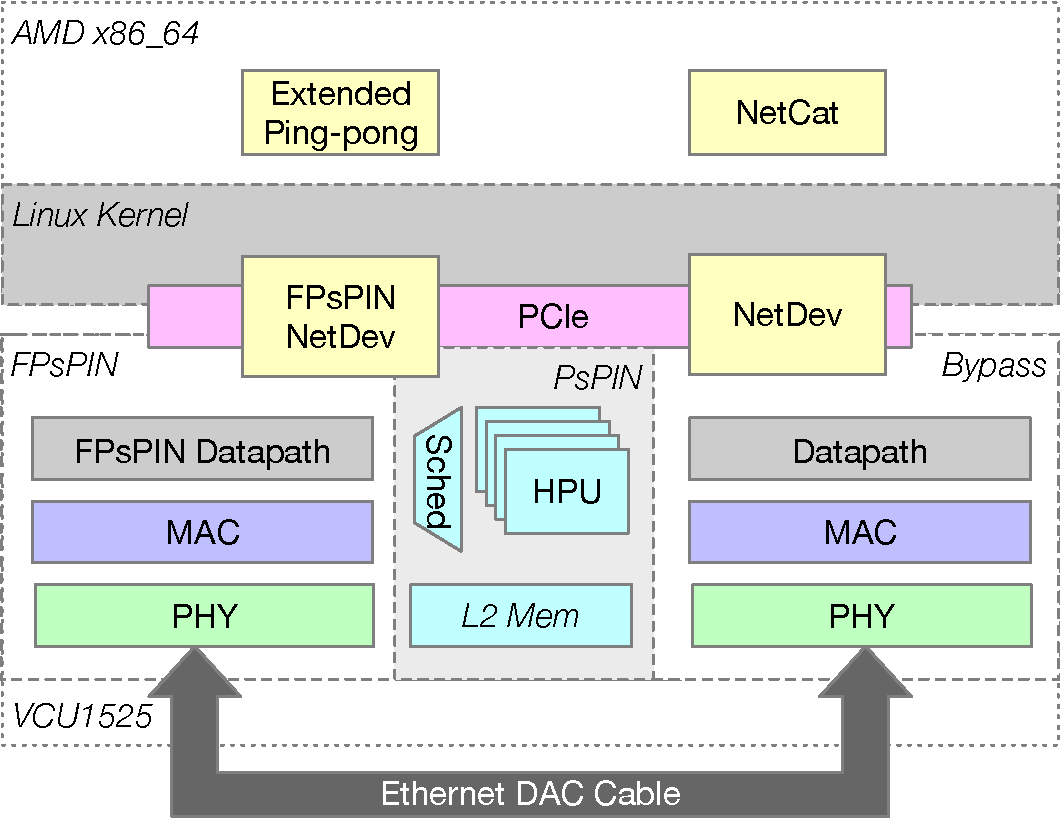
\includegraphics[width=.9\linewidth]{figures/experiment-setup.pdf}
    \caption{The experiment setup.  The host application of sPIN and the tester (\texttt{netcat} in the diagram) are in two separate network namespaces to prevent the direct loopback mechanism in Linux.}
    \label{fig:experiment-setup}
\end{figure}

\section{Theoretical data path analysis} \label{sec:hw-latency-analysis}

We estimate the latency of the hardware components as described in \Cref{sec:hw}.  \Cref{tab:lat-cycles} shows the latency in cycles based on the state machine construction in the Verilog RTL code, the frequency, and the latency time in nanoseconds.  Due to a limitation in the implementation, not all modules have a constant latency (\texttt{pspin\_ingress\_dma}), but is instead linearly related to the packet size.  We show in the next paragraph that these latency numbers are negligible compared to other parts of the system and, thus, would not have a big impact on overall latency.

\begin{table}[!htbp]
    \centering
    \begin{tabular}{lccc}
    \toprule
    Module & Cycles & Frequency (MHz) & Latency (ns) \\ \midrule
    Matching engine & 4 & 40 & 100 \\
    Allocator & 0 & 40 & 0 \\
    Ingress DMA & 8\mytilde{}70 & 40 & 200\mytilde{}1750 \\
    HER generator & 0 & 40 & 0 \\
    Host DMA & \emph{n/a} & 250 & \mytilde{}450 \\
    \bottomrule
    \end{tabular}
    \caption{Latency estimation for various data path modules in cycles and nanoseconds.  Note that as the host DMA goes over PCIe to the host DRAM, the exact latency in cycles is difficult to estimate; the latency in nanoseconds is measured on real hardware via the Integrated Logical Analyzer (ILA) on Xilinx platforms.}
    \label{tab:lat-cycles}
\end{table}

\section{Demo applications on real hardware}
We present two end-to-end demo applications to showcase that FPsPIN has realistic performance characteristics. We show that it is possible to write arbitrary packet-processing applications for the platform. The two applications follow the same operation workflow, also shown in \Cref{fig:demo-apps}:

\begin{enumerate}
    \item a packet comes in and matches for SmartNIC processing
    \item the cluster processes the packet
    \item (optionally), the cluster forwards it to the host for further processing
    \item the cluster sends back a response packet
\end{enumerate}

\begin{figure}
    \centering
    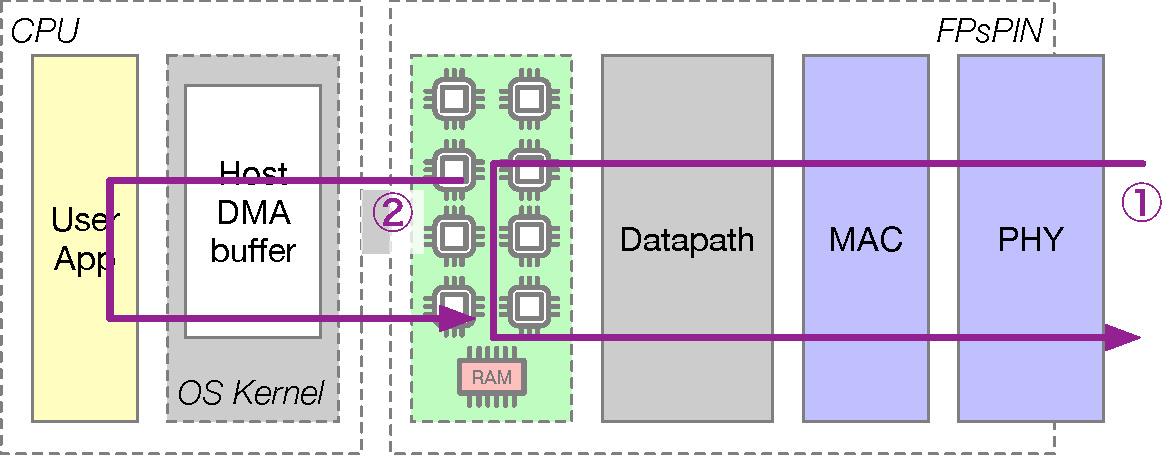
\includegraphics[width=.9\linewidth]{figures/demo-apps.pdf}
    \caption{Workflow of the demo applications.  The cluster can forward the packet to the host application for further processing, denoted with the red dashed arrow.}
    \label{fig:demo-apps}
\end{figure}

\pengcheng{the two pingpong demos are functional demos that exercise different components; slmp file transfer is a synthetic benchmark to measure throughput; datatypes show the overlapping, latency, and bandwidth characteristics of a real-world application}

\subsection{ICMP Echo ("ping")}

We evaluate the end-to-end system latency with the ICMP-Echo-Response test, also known as the \emph{ping} test.  For an ICMP payload size of 56 (the default value) and 1400 bytes, we evaluate two different scenarios:

\begin{itemize}
    \item Without host: the handler code swaps the IP address and Ethernet address of the incoming packet, sets the reply bit of the ICMP Echo packet and recalculates the ICMP checksum.
    \item With host: same as above, but the ICMP checksum calculation is performed on the host.
\end{itemize}

The resulting latency measurement is shown in \Cref{tab:icmp-ping}.  We notice that for small packets (56 B payload), FPsPIN shows performance on par with the host-only scenario; a further breakdown shows that half of the 33 us latency comes from the handler execution.  As explained in \Cref{sec:future-work}, one of the future works planned is to increase the $F_{\text{max}}$ of the design.  The projected latency of PsPIN, either with or without host processing, is then significantly better than the host-only case.

Another important purpose of SmartNICs is an offloading -- freeing precious CPU cycles from networking tasks.  Even though we notice slightly worse E2E latency for larger payloads, the on par results combined with the fact that the CPU can stay completely out of the reply processing and do other useful work.  This makes a compelling case for high-bandwidth scenarios to use FPsPIN for offloading communication tasks.

\begin{table}[!ht]
    \centering
    \begin{tabular}{clccc}
    \toprule
    Size (B) & Setup & E2E (us) & Handler (us) & Proj. E2E (us) \\ \midrule
    56 & H & \textbf{29} & \emph{n/a} & \emph{n/a} \\
    56 & P & 33 & 17 & {\color{acmgreen}\textbf{18}} \\
    56 & P+H & 37 & 21 & {\color{acmgreen}\textbf{19}} \\ \midrule
    1400 & H & \textbf{33} & \emph{n/a} & \emph{n/a} \\
    1400 & P & 264 & 244 & {\color{acmyellow}\textbf{59}} \\
    1400 & P+H & 124 & 104 & {\color{acmyellow}\textbf{36}}\\
    \bottomrule
    \end{tabular}
    \caption{Latency measurements of the ICMP ping handler under different operating scenarios: H denotes the baseline case (normal NIC, no PsPIN intervention; marked in bold); P denotes PsPIN-only; P+H denotes PsPIN and host together.  The size column denotes the ICMP payload size (\texttt{-s} argument in \texttt{ping(8)}).  The handler latency correspond to PsPIN running at 40 MHz.  The projected end-to-end latency scales the handler latency to 250 MHz, assuming the rest of the latency stays fixed.}
    \label{tab:icmp-ping}
\end{table}

\subsection{UDP ping-pong}

While the ICMP ping protocol allows good performance characterisations of FPsPIN, the demo application does not showcase what FPsPIN is capable of, due to the rigidity of the protocol: it mandates that the response payload must stay the same as the request.  The UDP ping-pong demo allows more flexibility by allowing the responder to send back arbitrary data.  We use OpenBSD \texttt{netcat} to start a UDP connection.  The packet handler in FPsPIN manipulates the payload by \emph{appending} an upper-case version of the payload to the old payload, recalculating necessary lengths and checksums, and sending the packet back.

\Cref{tab:udp-ping} shows the latency measurements of the UDP ping-pong demo.  We notice that the handler execution time aligns with that of ICMP ping in the case with host processing (18 us); the PsPIN-only setup showed even lower handler latency (5 us) due to UDP not requiring a payload checksum.  However, the end-to-end latency in the order of milliseconds show that the tester-side UDP stack added a significant amount of latency and measuring variance.  Nevertheless, the demo is still useful in demonstrating the capabilities of a PsPIN handler.

\begin{table}[!h]
    \centering
    \begin{tabular}{lcc}
    \toprule
    Setup & E2E (ms) & Handler (ms) \\ \midrule
    P & 5.1 & 0.005 \\
    P+H & 5.7 & 0.018 \\
    \bottomrule
    \end{tabular}
    \caption{Latency measurements of the UDP ping-pong handler.  We only measure PsPIN and PsPIN+Host setups due to a lack of an existing UDP ping-pong responder.}
    \label{tab:udp-ping}
\end{table}

\subsection{SLMP file transfer}

\pengcheng{parallel file receival - e2e bandwidth measurement}
\pengcheng{different operating modes (w/ and w/o ACK per msg or per packet) of SLMP}

\subsection{MPI datatypes} \label{sec:mpi-datatypes-demo}

\pengcheng{stress CPU with dgemm, tune size to minimise latency and poll overhead}
\pengcheng{overlapping ratio, e2e bandwidth and latency}
\pengcheng{message-level parallelism; 1. make handlers stateless; a) we replay segments on every packet b) ideally we get rid of the MPICH segments data structure with the compiled datatypes paper impl.  2. allocate dynamically the per-message state (to support arbitrary number of messages).  3. have a fixed number of message states for all in-flight messages and spill to the host if we have too many (picked)}